
\documentclass[border=8pt, multi, tikz]{standalone} 
\usepackage{import}
\subimport{E:/PlotNeuralNet-master/layers/}{init}
\usetikzlibrary{positioning}
\usetikzlibrary{3d} %for including external image 

\def\ConvColor{rgb:yellow,5;red,2.5;white,5}
\def\ConvReluColor{rgb:yellow,5;red,5;white,5}
\def\PoolColor{rgb:red,1;black,0.3}
\def\UnpoolColor{rgb:blue,2;green,1;black,0.3}
\def\FcColor{rgb:blue,5;red,2.5;white,5}
\def\FcReluColor{rgb:blue,5;red,5;white,4}
\def\SoftmaxColor{rgb:magenta,5;black,7}   
\def\SumColor{rgb:blue,5;green,15}

\newcommand{\copymidarrow}{\tikz \draw[-Stealth,line width=0.8mm,draw={rgb:blue,4;red,1;green,1;black,3}] (-0.3,0) -- ++(0.3,0);}

\begin{document}
\begin{tikzpicture}
\tikzstyle{connection}=[ultra thick,every node/.style={sloped,allow upside down},draw=\edgecolor,opacity=0.7]
\tikzstyle{copyconnection}=[ultra thick,every node/.style={sloped,allow upside down},draw={rgb:blue,4;red,1;green,1;black,3},opacity=0.7]

\node[canvas is zy plane at x=0] (input) at (0,0,0) {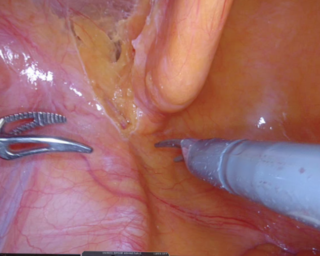
\includegraphics[width=7cm,height=7cm]{forcenet_input_frame.png}};

\pic[shift={(2.8,0,0)}] at (input-east) 
    {Box={
        name=conv1,
        caption=conv3d\\$7{\times}7{\times}7$\\64,
        xlabel={{64, }},
        zlabel=16,
        fill=\ConvColor,
        height=40,
        width=3,
        depth=40
        }
    };

\draw [connection]  (input-east)    -- node {\midarrow} (conv1-west);

\pic[shift={ (0,0,0) }] at (conv1-east) 
    {Box={
        name=pool1,
        caption=maxpool3d,
        fill=\PoolColor,
        opacity=0.5,
        height=32,
        width=2,
        depth=32
        }
    };

\draw [connection]  (conv1-east)    -- node {\midarrow} (pool1-west);

\pic[shift={ (2.2,0,0) }] at (pool1-east) 
    {RightBandedBox={
        name=layer1,
        caption=layer1\\$2{\times}$BasicBlock\\64,
        xlabel={{ 64, }},
        zlabel=16,
        fill={rgb:white,1;black,3},
        bandfill={rgb:white,1;black,2},
        opacity=0.2,
        height=30,
        width=6,
        depth=30
        }
    };

\draw [connection]  (pool1-east)    -- node {\midarrow} (layer1-west);

\pic[shift={ (2.4,0,0) }] at (layer1-east) 
    {RightBandedBox={
        name=layer2,
        caption=layer2\\$2{\times}$BasicBlock\\128,
        xlabel={{ 128, }},
        zlabel=8,
        fill={rgb:white,1;black,3},
        bandfill={rgb:white,1;black,2},
        opacity=0.2,
        height=24,
        width=5.5,
        depth=24
        }
    };

\draw [connection]  (layer1-east)    -- node {\midarrow} (layer2-west);

\pic[shift={ (2.4,0,0) }] at (layer2-east) 
    {RightBandedBox={
        name=layer3,
        caption=layer3\\$2{\times}$BasicBlock\\256 (tuned),
        xlabel={{ 256, }},
        zlabel=4,
        fill={rgb:white,1;black,3},
        bandfill={rgb:white,1;black,2},
        opacity=0.2,
        height=18,
        width=5,
        depth=18
        }
    };

\draw [connection]  (layer2-east)    -- node {\midarrow} (layer3-west);

\pic[shift={ (2.4,0,0) }] at (layer3-east) 
    {RightBandedBox={
        name=layer4,
        caption=layer4\\$2{\times}$BasicBlock\\512 (tuned),
        xlabel={{ 512, }},
        zlabel=2,
        fill={rgb:white,1;black,3},
        bandfill={rgb:white,1;black,2},
        opacity=0.2,
        height=13,
        width=4.5,
        depth=13
        }
    };

\draw [connection]  (layer3-east)    -- node {\midarrow} (layer4-west);

\pic[shift={ (2.0,0,0) }] at (layer4-east) 
    {Box={
        name=avgpool,
        caption=avgpool3d\\512,
        fill=\PoolColor,
        opacity=0.5,
        height=7,
        width=2,
        depth=7
        }
    };

\draw [connection]  (layer4-east)    -- node {\midarrow} (avgpool-west);

\pic[shift={(2.4,0,0)}] at (avgpool-east) 
    {Box={
        name=fc1,
        caption=fc 512\\ReLU+Drop,
        xlabel={{512, }},
        zlabel=1,
        fill=\ConvColor,
        height=4,
        width=2.5,
        depth=24
        }
    };

\draw [connection]  (avgpool-east)    -- node {\midarrow} (fc1-west);

\pic[shift={(2.4,0,0)}] at (fc1-east) 
    {Box={
        name=fc2,
        caption=output\\force $\hat{f}$ (N),
        xlabel={{" ","dummy"}},
        zlabel=1,
        fill=\SoftmaxColor,
        opacity=0.8,
        height=4,
        width=2.5,
        depth=8
        }
    };

\draw [connection]  (fc1-east)    -- node {\midarrow} (fc2-west);

\end{tikzpicture}
\end{document}
